\documentclass[conference]{IEEEtran}
\IEEEoverridecommandlockouts
% The preceding line is only needed to identify funding in the first footnote. If that is unneeded, please comment it out.
\usepackage{cite}
\usepackage{amsmath,amssymb,amsfonts}
\usepackage{algorithmic}
\usepackage{graphicx}
\usepackage{overpic}
\usepackage{textcomp}
\usepackage{
xcolor}

\def\BibTeX{{\rm B\kern-.05em{\sc i\kern-.025em b}\kern-.08em
    T\kern-.1667em\lower.7ex\hbox{E}\kern-.125emX}}

\usepackage[pagebackref=true,breaklinks=true,colorlinks,bookmarks=false]{hyperref}

\begin{document}

\title{Third Place in AICAS 2024  Challenge: From LLMs Compression to Deployment on ARM CPUs \\
% {\footnotesize \textsuperscript{*}Note: Sub-titles are not captured in Xplore and
% should not be used}
}

% 1\textsuperscript{st} 
\author{\IEEEauthorblockN{Ziqiang Chen}
\IEEEauthorblockA{
\textit{Zhejiang Lab}\\
Hangzhou, China \\
chenzq@mail.ustc.edu.cn}
\and
% 2\textsuperscript{nd}
\IEEEauthorblockN{Renhuang Huang}
\IEEEauthorblockA{
\textit{Ant Group}\\
Hangzhou, China \\
576788582@qq.com}
\and
%3\textsuperscript{rd}
\IEEEauthorblockN{Xuedian Hu}
\IEEEauthorblockA{
\textit{Zhejiang Lab}\\
Hangzhou, China \\
hxdsdu@163.com}

}

\maketitle

\begin{abstract}
The Large Language Models (LLMs) is widely employed for tasks such as intelligent assistants, text summarization, translation, and multi-modality on mobile phones. However, the current methods for on-device LLMs deployment maintain slow inference speed, which causes poor user experience. The AICAS 2024 conference hosts a performance optimization competition for LLMs inference, leveraging the ArmV9-based Yitian 710 CPU as the platform, with the aim of fostering technological research and development in this field. In our study, we introduced Log Relative Magnitude (LogRM) as a metric to assess the importance of layers in LLMs and proposed a pruning method that removes redundant layers based on their LogRM scores. We utilize the k-quants low-bit quantization method and develop high-performance matrix multiplication kernels using the new SIMD instruction set to accelerate LLM inference on ARM CPUs. Utilizing our proposed pruning method, low-bit quantization, and kernel optimization strategies, we have achieved an end-to-end inference throughput of 380 tokens/s during the prefill stage and 64 tokens/s in the generation stage for large models on an 8-core CPU. Prefill throughput outperforms PyTorch-based solutions by up to 4.38x, and decode throughput by up to 30.94x. Our approach's applicability is demonstrated through its application on Qwen-7B and Qwen-1.8B, showcasing exceptional inference efficiency on ARM CPUs, which led to a third-place finish in the finals. 
\end{abstract}

\begin{IEEEkeywords}
large language model, inference system, model compression, arm
\end{IEEEkeywords}

\section{Introduction}
Large Language Models (LLMs) have demonstrated exceptional proficiency in a wide array of natural language processing tasks, encompassing text comprehension, generation, sentiment analysis, machine translation, and interactive question answering~\cite{miao2023towards,touvron2023llama,code_llama_Rozière_Gehring_Gloeckle_Sootla_Gat_Tan_Adi_Liu_Remez_Rapin_et,qwen_1_8_bai2023qwen,zhang2022opt}. Despite their remarkable capabilities, the challenge of effectively deploying these models on edge devices is compounded by their massive parameter counts, which can reach into the billions or even trillions~
\cite{li2024transformer_lite}. Moreover, the exponential growth of model parameters has outpaced the advancements in hardware performance, prompting both academic and industrial sectors to seek innovative solutions~\cite{miao2023towards,alizadeh2023llm_flash}.

These solutions include model compression techniques~\cite{shortgpt_Men_Xu_Zhang_Wang_Lin_Lu_Han_Chen,slicegpt_ashkboos2024slicegpt}, dataflow optimizations, and operator invocation strategies to facilitate the deployment and operation of large-scale models within the constraints of limited hardware resources.

The escalating demand for edge deployment of large models, coupled with the diverse nature of computing resources, has made the deployment of these models on CPU architectures a pivotal area of development~\cite{arm_cpu_llms,intel_cpu_Shen_Chang_Dong_Luo_Meng_2023,li2024transformer_lite}. The prevalence of Arm-based CPUs in edge devices has further underscored the significance of this focus. In light of this,  AICAS 2024 has designated the ArmV9-based Yitian 710 CPU as the computational platform for a comprehensive large model performance optimization competition. This initiative is designed to stimulate and enhance technological research and development in this domain.

While the initial phase of the competition does not mandate specific hardware platforms, our team has strategically chosen to employ CPU hardware platforms for optimizing the inference performance of large models. This decision is driven by the competition's objectives and an anticipation of the finals' content. Our efforts are concentrated on Algorithm Innovation and System Optimizations, which encompass a range of strategies such as model compression, low-bit quantization, parallel computing, memory management, operator kernel enhancement, and decoding algorithm refinement. These approaches are aimed at maximizing the efficiency and effectiveness of large model deployment and execution on CPU architectures, thereby propelling the frontiers of computational linguistics and artificial intelligence.


\begin{figure}
    \begin{overpic}[width=\columnwidth]{taxonomy.png}
    \end{overpic}
    \caption{The modules highlighted with a red flag indicate the specific areas that our team is prioritizing for optimization.}
    \label{fig:taxonomy}
\end{figure}

\section{Background}

\subsection{Transformer-based LLM}

Transformer-based LLMs have brought about a significant shift in the field of natural language processing, introducing a new paradigm for understanding and generating human language. At the core of this innovation lies the Transformer architecture, which is founded on the concept of self-attention mechanisms~\cite{self_attention_Vaswani_Shazeer_Parmar_Uszkoreit_Jones_Gomez_Kaiser_Polosukhin_2017}, enabling the model to assess the significance of various parts of the input data when making predictions. Mathematically, the self-attention mechanism in Transformers can be described as follows: For an input sequence $X = [x_1,x_2,...,x_n]$, the Transformer computes a set of queries $Q$, keys $K$ and values $V$ using linear transformations of $X$ . The self-attention scores are then computed as:

%% self-attention
\begin{equation}
Attention(Q,K,V)=softmax(\frac{QK^T}{\sqrt{d_k}})
\label{eq:self_attention}
\end{equation}

where $d_k$ is the dimension of the keys. This mechanism allows the model to focus on different parts of the input sequence for each element of the output, capturing complex dependencies regardless of their distance in the input sequence.

A transformer consists of multiple Multi-Layer Perceptron (MLP) and Attention blocks. The design of MLP and Attention can be different for each model. Transformer is a sequence to sequence mapping, which can be defined as $y = f(X,\theta)$, where $X \in R^{S\times n}$, $Y \in R^{S\times n}$, $S$ is the length of the sequence, $n$ is the vocabulary size, $\theta$ is the learnable parameters. The formal expression of an L-layer transformer is as follows:

%% transformer block
\begin{gather}
\mathbf{X}_0 = \mathbf{X}\mathbf{W}_{emb} \notag \\
\mathbf{A}_{i+1} = ATTN(LN(\mathbf{X}_i)) + \mathbf{X}_i \notag \\
\mathbf{X}_{i+1} = MLP(LN(\mathbf{A}_{i+1})) + \mathbf{A}_{i+1} \notag \\
\mathbf{Y} = \mathbf{X}_{L}\mathbf{W}_{head}
\label{eq:transformer}
\end{gather}

where $\mathbf{W}_{emb} \in R^{n\times d}$ is the word embedding matrix, $\mathbf{W}_{head} \in R^{d \times n}$ is the output projection matrix of the transformer, which are sometimes tied with the $\mathbf{W}_{emb}$, $d$ is the hidden dim of the transformer. $ATTN$ refers to the attention and $MLP$ means the multiple Multi-Layer perceptron, $\mathbf{X}_i \in R^{T \times d}$ is the hidden states of the $i^{th}$ layers.

An inference request to a transformer model consists of a prompt and is served in two phases: (i) \textit{prefill processing}, where the prompt is processed, and (ii) \textit{token generation}, where a series of tokens that represents the output response text is generated incrementally. The model can batch $B$ requests into a single inference task. The sequence length $S$ denotes the number of tokens of each request being processed in the prefill processing phase or the number of tokens of each request being generated in the token generation phase. Therefore, during prefill processing $B \geq 1, S \geq 1$ and during token generation $B \geq 1, S = 1$.

\begin{figure*}[!t]
\centering
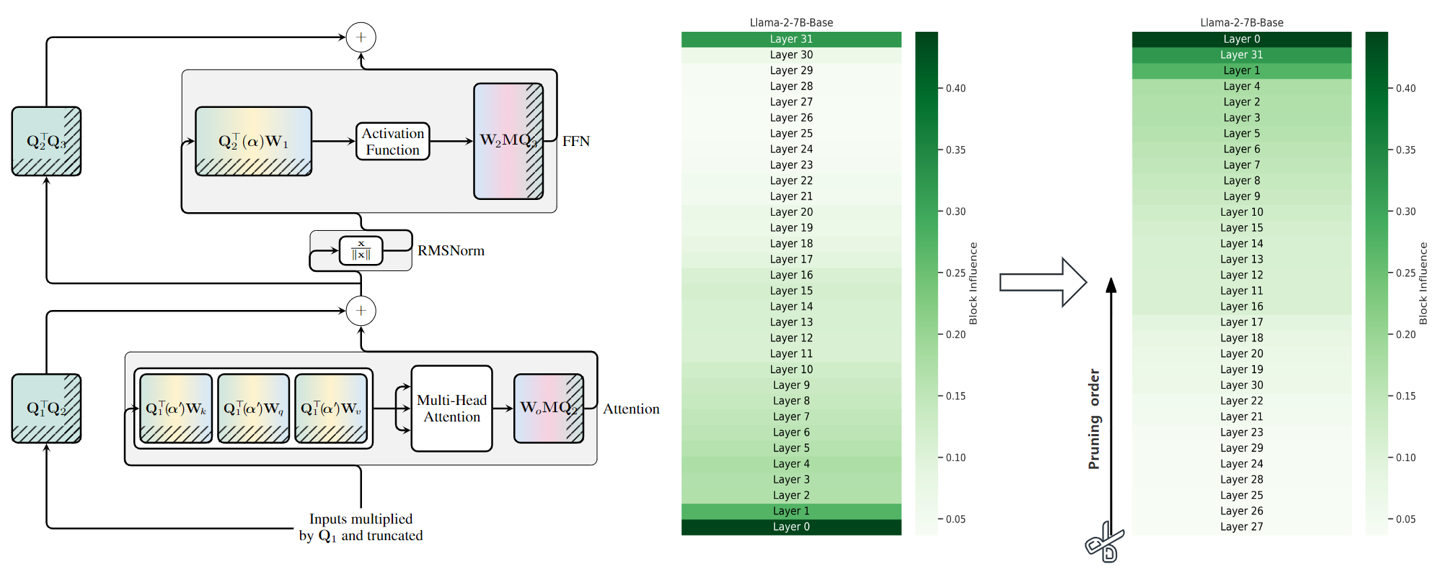
\includegraphics[width=\textwidth]{slice_short.png} 
\caption{Left: SliceGPT - Making LLMs Leaner, Right: ShortGPT - Making LLMs Shorter.}
\label{fig:slice_short}
\end{figure*}

\subsection{Efficient LLM Inference on CPUs}

In the realm of artificial intelligence and machine learning, CPUs are increasingly being acknowledged for their prowess in handling inference tasks for large language models (LLMs). While GPUs are renowned for their parallel processing capabilities, CPUs offer distinct advantages owing to their architectural design, which excels in intricate control, decision-making, and context management. Modern CPUs, equipped with advanced instruction sets and enhanced vector processing, are well-suited for the matrix operations central to LLM inference. Intel's Advanced Matrix Extensions (AMX), for instance, bolster vector operation performance, rendering CPUs a competitive choice for neural network computations.

Despite GPUs' superior floating-point operations per second (FLOPs), CPUs provide a cost-effective alternative for inference, especially when considering operational costs and energy efficiency~\cite{intel_cpu_Shen_Chang_Dong_Luo_Meng_2023}. The ample cache capacity of CPUs proves beneficial for caching key-value pairs, a crucial optimization in transformer-based models, potentially reducing memory access latency and expediting inference. As technology progresses, CPUs are anticipated to become even more competitive in AI, offering a balanced and energy-efficient approach to LLM inference tasks. Moreover, LLMs are often BW bound and have a large weight memory footprint – CPU can achieve competitive performance. Llama.cpp (GGML) c/c++ runtime demonstrates performance on existing Arm platforms but fails to demonstrate the true potential of Arm CPUs~\cite{arm_cpu_llms}. 

\subsection{Challenges}
\begin{itemize}
\item \textbf{Latency and Response Time.} Efficient inference in large language models is essential for real-time applications such as chatbots and virtual assistants, where low latency and swift response are paramount. Balancing model complexity with inference speed is a critical challenge that necessitates optimizing algorithms and system architectures to minimize response time without compromising accuracy.
\item \textbf{Memory Footprint and Model Size.} 
Large language models, with their extensive memory demands due to substantial parameter counts, present a deployment challenge on devices with limited memory. This requires the implementation of sophisticated model compression strategies and system enhancements to maintain performance while significantly shrinking the memory footprint.
\item \textbf{Scalability and Throughput.} Inference systems must contend with fluctuating request volumes in production settings. To ensure scalable and high-throughput processing of concurrent requests, it is imperative to implement parallel computation and efficient request scheduling, alongside other system-level optimizations. These measures facilitate the optimal distribution of computational workloads across available resources.
\item \textbf{Trade-offs between Accuracy and Efficiency.} Optimizing the efficiency of LLM inference may sometimes involve trade-offs with model accuracy. Striking the right balance between model size, computational complexity, and performance is a challenging task that requires careful consideration and evaluation of various algorithmic and system-level techniques.
\end{itemize}


\section{Our Approach}

Considering these challenges and the prevailing landscape of CPU-based inference for large models, our primary optimization efforts are concentrated in two key areas: \textbf{Algorithm Innovation} and \textbf{System Optimizations}. Specifically, this includes model compression, model sparsification, low-bit quantization, parallel computing, memory management, operator kernel optimization, decoding algorithm optimization, and more.

%%%%%%%%%%%%%%%%%%%%%%%%%%%%%%%%%%%%%%%%%%%%%%%%%%%%%%%%%%%%
%%%%%%%%%%%%%%%%%%%%%%%%%%%%%%%%%%%%%%%%%%%%%%%%%%%%%%%%%%%%
% Model Compression

\subsection{Model Compression}\label{AA}
Model compression aims to reduce the memory footprint and computational requirements of LLMs by creating more efficient and compact models without significant loss in performance.  A majority of model compression techniques fall into one of four categories: distillation, tensor decomposition (which includes low-rank factorization), pruning and quantization. Pruning provides a solution to alleviate these resource constraints, and recent works have shown that trained models can be sparsified post-hoc.

Sparsification stands as an essential technique that aims to alleviate the storage and computational burdens associated with neural network models, all while preserving their efficacy. Our team has identified and adopted two state-of-the-art (SOTA) algorithms in this field: SliceGPT~\cite{slicegpt_ashkboos2024slicegpt} and ShortGPT~\cite{shortgpt_Men_Xu_Zhang_Wang_Lin_Lu_Han_Chen}. These algorithms epitomize distinct methodologies for pruning large models along both vertical and horizontal axes.

\begin{itemize}
    \item \textbf{SliceGPT: The Art of Parameter Slicing.} SliceGPT targets the essence of model sparsification by identifying and removing low-impact parameters, grounded in the concept of parameter importance. This method leverages parameter significance analysis to streamline the model, maintaining its predictive power while reducing its complexity.
    \item \textbf{ShortGPT: Streamlining Neural Structure.} ShortGPT focuses on structural efficiency, trimming the neural network's architecture by reducing layer counts. This approach is rooted in controlling model complexity to prevent overfitting, ensuring generalization. ShortGPT also employs strategies like parameter sharing and quantization for additional model compression.
\end{itemize}

ShortGPT discovered that many layers of LLMs exhibit high similarity, and some layers play a negligible role in network functionality. In 
\cite{rm_Samragh_Farajtabar_Mehta_Vemulapalli_Faghri_Naik_Tuzel_Apple,shortgpt_Men_Xu_Zhang_Wang_Lin_Lu_Han_Chen}, they proposed to use relative magnitude (RM) or Block Influence (BI) to measure the importance of layers. Based on this observation, we define a new metric called Log Relative Magnitude (LogRM) to gauge the significance of each layer in LLMs, which performs better on Qwen-1.8B~\cite{qwen_1_8_bai2023qwen}.

%% log relative magnitude
\begin{gather}
RM = ||\frac{f(x)}{x+f(x)}||  \\
BI = 1 - \frac{\mathbf{X}_i^T\mathbf{X}_{i+1}}{||\mathbf{X}_i||_2 ||\mathbf{X}_{i+1}||_2} \\
LogRM = abs(log(\frac{||\frac{f(x)}{x+f(x)}||}{1 - ||\frac{f(x)}{x+f(x)}||}))
\label{eq:log_rm}
\end{gather}

Suppose we aim to prune four transformer layers from the Qwen-1.8B model, guided by indicators of layer importance, followed by an assessment of the model's performance using three distinct metrics(RM, BI, LogRM) on the PIQA dataset. The anticipated outcomes of this process are as follows table~\ref{tab:import_index}.

\begin{table}[htbp]
\caption{Setup of Removed Layers for Qwen-1.8B and Comparison of Strategies for Layer Removal on PIQA.}
\begin{center}
\begin{tabular}{|c|c|c|}
\hline
Method & Removed Layers & PIQA \\ \hline
RM ~\cite{rm_Samragh_Farajtabar_Mehta_Vemulapalli_Faghri_Naik_Tuzel_Apple} & 7,9,8,10 & 0.6630 \\ \hline
BI ~\cite{shortgpt_Men_Xu_Zhang_Wang_Lin_Lu_Han_Chen} & 20,21,22,11 & 0.6512 \\ \hline
LogRM (ours) & 10,11,9,12 & \textbf{0.6908} \\ \hline
\end{tabular}
\label{tab:import_index}
\end{center}
\end{table}

\begin{table}[tbp]
\caption{Comparison of pruning methods on PIQA. In ShortGPT-N, 'N' refers to the number of pruned block layers.}
\begin{center}
\begin{tabular}{|c|c|c|}
\hline
Method & Memory (MB) & PIQA \\ \hline
Dense(F16) & 3503 & 0.733 \\ \hline
SliceGPT(15\%) & 2999 & 0.659 \\ \hline
SliceGPT(25\%) & 2625 & 0.611 \\ \hline
ShortGPT-2 & 3300 & 0.712 \\ \hline
ShortGPT-4 & 3000 & 0.691 \\ \hline
\end{tabular}
\label{tab:pruning_method}
\end{center}
\end{table}

Our empirical evaluation on the PIQA test suite has led us to favor ShortGPT for model sparsification. The comparative result from our experiments is presented in the accompanying table~\ref{tab:pruning_method}. It is important to note that the principles underlying these two techniques are complementary, allowing for their synergistic application to further enhance model efficiency. 

%%%%%%%%%%%%%%%%%%%%%%%%%%%%%%%%%%%%%%%%%%%%%%%%%%%%%%%%%%%%
%%%%%%%%%%%%%%%%%%%%%%%%%%%%%%%%%%%%%%%%%%%%%%%%%%%%%%%%%%%%
% Low-bit Quantization

\subsection{Low-bit Quantization}\label{BB}

\begin{table}[htbp]
\caption{Comparison of k-quants methods on Qwen-1.8B}
\begin{center}
\begin{tabular}{|c|c|c|}
\hline
Method   & Memory (MB) & PIQA   \\ \hline
Dense(FP16)     & 3420.0       & 0.7312 \\ \hline
Q2\_K    & 791.9       & 0.6502 \\ \hline
Q4\_0    & 1040.0       & 0.7144 \\ \hline
Q4\_K\_M & 1150.0       & 0.7198 \\ \hline
Q8\_0    & 1820.0       & 0.7265 \\ \hline
\end{tabular}
\label{tab:k_quants}
\end{center}
\end{table}

Low-bit quantization techniques provide an efficient means of encoding model weights and activation values, utilizing fewer bits than the conventional 32-bit precision to represent numerical data. This approach markedly decreases memory requirements and enhances the speed of inference processes on various hardware platforms. The primary strategies within quantization are succinctly divided into two categories: Quantization-Aware Training (QAT) and Post-Training Quantization (PTQ). Specifically, PTQ employs tailored kernels to decrease the precision of model weights and activations to INT8 or INT4, thereby achieving a balance between performance and computational efficiency. 

\begin{figure}[htbp]
    \begin{overpic}[width=\columnwidth]{q_40_80.png}
    \end{overpic}
    \caption{Block Quantized Formats}
    \label{fig:q8_0_q4_0}
\end{figure}

We have adopted the K-quants~\cite{k_quants_github_repository} quantization method, implemented in llama.cpp, as a Post-Training Quantization (PTQ) technique for neural network models. Its objective is to reduce model size and enhance operational efficiency while maintaining model performance. The K-quants quantization method achieves model compression by reducing the bit-width of model parameters to between 2 and 8 bits. This approach provides a variety of quantization strategies, allowing users to select the optimal quantized model based on their computational resource limitations, such as memory capacity and inference speed. The essence of quantization is to map continuous weight parameters to a finite set of discrete values, thereby reducing storage requirements and computational complexity of the model. Llama.cpp/GGML use block quantized formats to store chunks of weight columns and activations, as shown in the figure~\ref{fig:q8_0_q4_0}.

In our evaluation, we examined a variety of quantization techniques, specifically focusing on Q2\_K, Q4\_0, Q4\_K\_M, and Q8\_0, as applied to the Qwen-1.8B model. We conducted a comprehensive comparison based on several key metrics, including the count of parameters, memory footprint, and performance discrepancies as measured by the PIQA metric. The synthesized findings are succinctly presented in the table~\ref{tab:k_quants}.


\subsection{Kernel Optimization}\label{CC}

\begin{figure}
    \begin{overpic}[width=\columnwidth]{perf-llamacpp.png}
    \end{overpic}
    \caption{ARM CPU Flame Graph}
    \label{fig:fire}
\end{figure}

\begin{figure*}[!t]
\centering
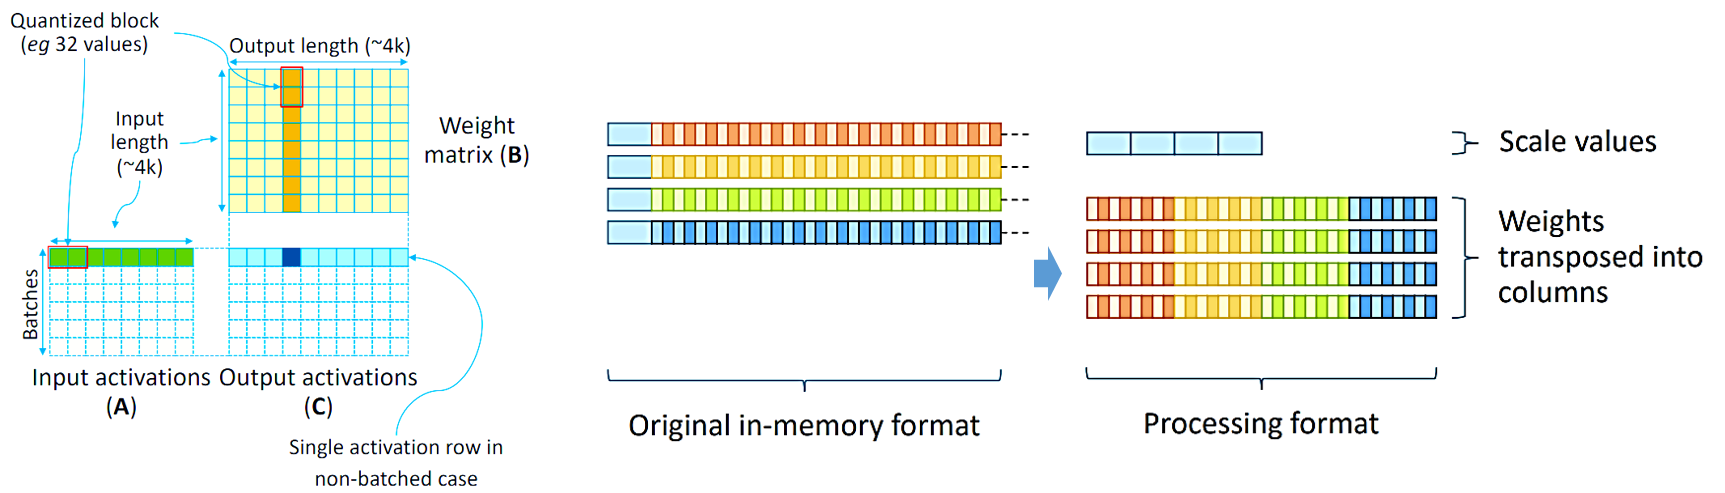
\includegraphics[width=\textwidth]{gemm_kernel2.png} 
\caption{To avoid pseudo-scalar operations, rearrange parameters in the weight matrix.}
\label{fig:gemm_kernel}
\end{figure*}

Through testing on ARM CPUs, we found that the GEMV and GEMM kernels play a crucial role in the Qwen-1.8B inference process, as shown in illustration~\ref{fig:fire}, constituting a higher proportion. We concentrate on leveraging more powerful computing instructions and selecting SIMD instruction sets with higher computational peaks to expedite core calculations, particularly in accelerating matrix multiplication operations.

Armv8.6-A has introduced general matrix multiply (GEMM) instructions to both SVE and NEON instruction sets, which reduce memory access and increase computation compared to previous multiplication and multiply-accumulate instructions. In LLM inference, GEMM constitutes a very high computational workload, so utilizing the new instructions in ARMv8.6-A can significantly enhance model inference performance. These instructions have theoretically double the performance capability of ARMv82sdot; using them for int8 matrix multiplication can bring about a substantial performance boost. This article presents an implementation of the MatMul operator using the new instructions from ARMv86, achieving up to approximately 150\% performance improvement in prompt calculations. 

For typical operators in LLMs, weight matrix (B) is much larger than the input (A) and output (C), as shown in the GEMM on the left side of the figure~\ref{fig:gemm_kernel}. Compression of weight matrix is key to reducing memory and bandwidth consumption. In GGML, a dot-product kernel computes a single result – it’s called at each point to populate the whole of C.

Half of the operations in the original code are scalar or 'pseudo-scalar', operating on a vector of values that are essentially one true value split across lanes. To circumvent the inefficiencies associated with pseudo-scalar operations, we rearrange parameters in the weight matrix. Rather than permuting weights on each iteration, we adopt a blocked memory format for storage, as shown  on the right side of the figure~\ref{fig:gemm_kernel}. This approach embodies the space-time tradeoff paradigm in computer science, enhancing performance through the strategic allocation of memory resources at the expense of increased memory usage. As a result~\ref{tab:performance}, we increased the throughput of the prefill stage to 380 token/s, but our memory usage also increased by nearly one-third because we stored the same parameter data in a different order.


\subsection{Speculative Decoding}\label{DD}

In LLM inference, traditional autoregressive sampling methods decode tokens sequentially, leading to slow computational processes due to memory access limitations. Speculative sampling techniques address this by adjusting the computation-to-memory access ratio while maintaining the model's sampling distribution. This approach employs a dual-model framework: a large target model and a smaller, more efficient approximate model. The smaller model handles straightforward token generation, while the larger model evaluates outcomes, reducing computational load and memory access requirements.

Our research focuses on Prompt Lookup Decoding~\cite{saxena2023prompt_lookup}, a speculative sampling strategy that accelerates generation in large models. Particularly effective for tasks like summarization, content-based question answering, and multi-turn dialogues, where content primarily derives from prompt inputs. By replacing the small model with a content lookup function during speculative sampling, Prompt Lookup Decoding significantly enhances generation speed and simplifies the inference process.


\section{Results}

\begin{figure}[htbp]
    \begin{overpic}[width=\columnwidth]{radar.png}
    \end{overpic}
    \caption{Performance of different model sparsification and quantization methods. The increase in memory space resulting from the rearrangement of the weight matrix is traded for enhanced prefill throughput, denoted as \textbf{+RW}}
    \label{fig:radar}
\end{figure}

\subsection{System}\label{4_1}

Our experimental setup utilized an ARM CPU (Yitian 710) supplied by the event organizers, which boasted a 8-core CPU, 30GB of memory, and 50GB of disk space. Meanwhile, in compliance with the competition's specifications, we validated our optimization method using the Qwen-1.8B~\cite{qwen_1_8_bai2023qwen}. We evaluate the accuracy of both Q4\_0 and Q8\_0 models using open-source datasets from lm-evaluation-harness~\cite{lm_eval_harness} including PIQA~\cite{bisk2020piqa} task.
To assess performance, we measure the resident set size ($M_{RSS}$), virtual memory usage ($M_{VMS}$), throughput of the prefill stage ($T_{pre}$), and throughput of the decode stage ($T_{dec}$). After normalizing each metric separately, calculate the final score using the following formula ~\ref{eq:score_calc}.

%% final-score calc
\begin{equation}
\begin{split}
Score &= Acc \cdot 0.30 + {{RSS}} \cdot 0.15 + {{VMS}} \cdot 0.15 \\ &\quad  +  {{Pre}} \cdot 0.15 + {{Dec}} \cdot 0.25
\end{split}
\label{eq:score_calc}
\end{equation}

\subsection{Accuracy}\label{4_2}

\begin{table}[htbp]
\caption{Prediction accuracy of differently sparsed Qwen-1.8B models under various quantization methods. In Short-N, 'N' refers to the number of pruned block layers.}
\begin{center}
\begin{tabular}{|c|c|c|c|c|}
\hline
Quant Type & Qwen-1\_8B & Short2 & Short4 & Short5 \\ \hline
Q4\_0    & 0.7144     & 0.7084            & 0.6823            & 0.6910            \\ \hline
Q8\_0    & 0.7285     & 0.7255            & 0.7160            & 0.7188            \\ \hline
\end{tabular}
\label{tab:accuracy}
\end{center}
\end{table}

We evaluate the accuracy on the aforementioned datasets and show the average accuracy in Table~\ref{tab:accuracy}. The prediction accuracy after Q8\_0 quantization is higher than that of Q4\_0. To balance the prediction accuracy, we prefer to use Q8\_0 for quantization whenever possible. The number of removed layers affects prediction accuracy; generally, more layers removed leads to greater accuracy loss. However, with proper fine-tuning, we can improve the degraded precision.

\subsection{Performance}\label{4_3}

We optimized our inference system based on the llama.cpp project. To evaluate the post-optimization performance, we used a 560-tokens text input to generate 50 tokens, measuring the aforementioned performance metrics during this process. We conducted 10 measurements and took the average for each metric, with the results presented in the table ~\ref{tab:performance}.

\begin{table}[htbp]
\caption{LLM prefill throughput outperforms PyTorch-based solution by up to 4.38x under Short5-Q8\_0+RW.}
\begin{center}
\begin{tabular}{|c|c|c|c|c|c|c|}
\hline
Model           & PIQA            & RSS           & VMS           & Prefill         & Decode         & Score          \\ \hline
Short2-Q4\_0    & 0.7084          & 1180          & 1276          & 121.69          & 49.65          & 60.05          \\ \hline
Short2-Q8\_0    & \textbf{0.7255} & 1970          & 2064          & 140.93          & 52.01          & 67.86          \\ \hline
Short4-Q4\_0    & 0.6823          & \textbf{1132} & \textbf{1227} & 134.34          & 52.66          & 47.29          \\ \hline
Short4-Q8\_0    & 0.7160          & 1835          & 1930          & 163.67          & 55.47          & 64.62          \\ \hline
Short5-Q8\_0    & 0.7187          & 1775          & 1849          & 175.55          & 56.18          & 66.74          \\ \hline
Short5-Q8\_0+RW & 0.7188          & 2756          & 2871          & \textbf{380.61} & \textbf{64.05} & \textbf{70.66} \\ \hline
\end{tabular}
\label{tab:performance}
\end{center}
\end{table}


\section{Summary and Future Work}

We presented an end-to-end LLM inference including model compression, low-bit model quantization and efficient kernel optimization. We demonstrated the performance advantage over the open-source solution on ARM CPUs. As our future works, we plan to further improve the ARM CPU tensor library to support LLM inference as part of the contributions to the open-source community. Moreover, leveraging the ubiquity of CPUs, we intend to extend our methodology to edge devices, aiming to satisfy the escalating demand for AI-generated content and augment the capacity for AI computation on ARM CPUs.

\section*{Acknowledgment}

We extend our sincere thanks to the competition organizers of AICAS 2024 and the Alibaba Cloud Tianchi Competition platform for their exceptional support and contributions.

%\bibliographystyle{ieee}
%\bibliography{REF}
\bibliographystyle{IEEEtran}
\bibliography{REF}

% \appendix 

% \subsection{Finetune Qwen-1.8B}\label{A_1}
% test

% \subsection{Model Compression}\label{A_2}
% test

% \subsection{Low-bit Quantization}\label{A_3}
% test

% \subsection{Reproduce Results}\label{A_4}
% test

\end{document}
